\documentclass[a4paper,11pt]{article}
\usepackage[margin=1in]{geometry}
\usepackage{amsmath,amssymb}
\usepackage{graphicx,xcolor,booktabs,array}
\graphicspath{{sample2036/}{report/sample2036/}}
\usepackage[hidelinks]{hyperref}
\urlstyle{same}
\setlength{\parindent}{1em}
\setlength{\parskip}{3pt}
\setlength{\emergencystretch}{2em}
\definecolor{policyA}{HTML}{D55E00}
\definecolor{policyB}{HTML}{0072B2}
\definecolor{policyAB}{HTML}{009E73}
\definecolor{baseline}{HTML}{666666}
\hypersetup{pdftitle={Can Alternating Weed-Control Policies Reverse an Increase in Infestation?},pdfauthor={Ray You and Kaz Morita}}
\begin{document}


\begin{center}{\large\bfseries Can Alternating Weed-Control Policies Reverse an Increase in Infestation?}\end{center}

\begin{center}CITS4403 Research Project\\Ray You and Kaz Morita\end{center}

\section{Background and Research Aims}

\subsection{Weed management and Parrondo's paradox}

Invasive weeds can damage native ecosystems and increase management costs. Weeds are not spread evenly across a landscape: some places are heavily infested, while others have few weeds. Managers therefore need to decide where and when to remove weeds with the resources available. Western Australian bushland guidance recommends protecting healthy vegetation and treating small or isolated infestations to limit further spread \cite{bushland}. This guidance provides a reason to consider the location of treatment. It does not prescribe the two model policies used in this study.

Following this idea, we compare two ways to choose treatment locations. Policy A treats the most heavily infested cells. Policy B treats cells in a lower infestation range that may spread weeds to their neighbours. With limited resources, either policy alone may fail to keep up with growth and spread. However, using one policy changes the landscape that the next policy encounters. Their combined result may therefore differ from what their separate results suggest.

This leads to the idea of Parrondo's paradox: two strategies that lose when used separately can win when combined \cite{parrondo}. We ask whether a similar reversal can occur in this weed model. Here, a strategy wins if the average infestation index ends below its starting value after a fixed number of steps. It loses if the index ends above that value. These terms describe change in the model, rather than profit or complete weed removal.

The same question fits a complex-systems approach. Each cell changes through local growth, spread from neighbours and treatment. These local changes affect which cells can be treated later, and together they determine the result for the whole region. As a result, alternating two policies need not produce the average of their separate outcomes. This is a reason to test for a reversal, rather than evidence that a reversal must occur.

\subsection{Research aims and approach}

To investigate this question, we first built a two-dimensional cellular automaton (CA) for weed growth, spread and removal. We then defined the two policies and compared four strategies: no treatment (Baseline), A only, B only and alternating AB. Finally, we examined a saved parameter search and ran further experiments on the Step 08 candidate with additional schedule-control evidence. Our contribution is to identify a reversal in this spatial model and test some possible explanations and limits. The model has not been fitted to observed weed abundance, so its results are not a forecast for Perth or a recommended field-management plan.

\section{Model Specification and Policy Definitions}

\subsection{Spatial state and initialisation}

Locality polygons from Landgate \cite{landgate} and 2021 Census population data from the Australian Bureau of Statistics \cite{abs} define the spatial input. The loader joins population to postcode-level land area and assigns that density to localities. We select postcodes 6000-6199 as an operational study region, without claiming an exact official metropolitan boundary. Rasterisation in EPSG:7850 produces 1 km square cells, including 6,933 valid cells in a 203 by 124 grid. Cells outside the selected land area are excluded.

Each valid cell was assigned a Weed Index ranging from 0 to 1, representing the relative level of weed infestation. The state of cell $i$ at timestep $t$ is $W_i^t\in[0,1]$. The Weed Index is treated as a relative modelling quantity rather than a direct measurement of plant biomass or weed density.

The initial spatial distribution of weed infestation was modelled using an exponential decay function:

\begin{equation}
W_i^0=W_{\min}+(W_{\max}-W_{\min})e^{-kD_i}.
\label{eq:initial}
\end{equation}

Here, $D_i$ is the population density associated with cell $i$, $k$ is the pressure coefficient, and $W_{\min}$ and $W_{\max}$ define the minimum and maximum initial Weed Index. We use $W_{\min}=0.05$, $W_{\max}=1$ and $k=0.000783$. Population density was calculated as population divided by the corresponding land area and used as a proxy for anthropogenic pressure. Under this modelling assumption, higher population density results in a lower initial Weed Index, reflecting the hypothesis that areas experiencing greater human activity are subject to stronger weed suppression or management. This assumption has not been fitted to weed observations. The initial regional mean is 0.860575.

\subsection{Growth and propagation}

Natural growth was represented using a discrete-time logistic growth model. When the Weed Index is relatively low, the growth increment is approximately proportional to the current Weed Index. As the Weed Index approaches the carrying capacity, the growth rate decreases, representing a saturation effect. The growth increment and updated state are
\begin{align}
G_i^t &= rW_i^t\left(1-\frac{W_i^t}{K}\right),\label{eq:growth}\\
W_i^{t,\mathrm{growth}} &= W_i^t+G_i^t.
\end{align}
Here, $r$ controls the growth rate and $K=1$ is the model-defined upper bound, rather than a directly measured ecological carrying capacity. One step represents one model update; a conversion to weeks would require observed growth data.

Spatial propagation was modelled using an eight-neighbour interaction structure. For each cell, the Weed Index was propagated only from neighbouring cells with a higher Weed Index to cells with a lower Weed Index. Let $N_8(i)$ denote the set of up to eight neighbouring cells. The propagation increment and updated state are
\begin{align}
D_i^t &= \alpha\sum_{j\in N_8(i)}\max\left(W_j^{t,\mathrm{growth}}-W_i^{t,\mathrm{growth}},0\right),\label{eq:spread}\\
W_i^{t,\mathrm{prop}} &= W_i^{t,\mathrm{growth}}+D_i^t.
\end{align}
Here, $\alpha$ controls the strength of spatial propagation. The superscript $\mathrm{growth}$ makes explicit that the implementation calculates propagation after natural growth. This formulation represents directional spatial propagation rather than classical mass-conserving diffusion: it increases lower-index cells without reducing neighbouring source cells. Grid edges do not wrap, invalid neighbours are excluded, and each growth and propagation update is restricted to $[0,1]$ in the implementation.

\subsection{Management policies and budget}

At each timestep, the model sequentially applies natural growth, spatial propagation, and management removal. The removal process is defined through a user-specified policy function, allowing different management strategies to be evaluated without modifying the underlying Cellular Automaton structure. If $R_i^t$ is the removal applied to cell $i$, the final state is
\begin{equation}
W_i^{t+1}=W_i^{t,\mathrm{prop}}-R_i^t.
\end{equation}
This policy-based structure separates management decisions from the underlying CA dynamics.

For the policy definitions, write $X_i=W_i^{t,\mathrm{prop}}$. Policy A selects cells with $X_i\geq h$, ranks them by decreasing index, and treats at most $m$ cells. It removes fraction $a$ of each selected index. For example, $a=0.2$ removes 0.16 from a selected cell with $X_i=0.8$. This is a model comparison rule, rather than a priority prescribed by the local guidance.

Policy B considers cells with $\ell\leq X_i<h$. For each candidate, it calculates an outward-spread score:
\begin{equation}
S_i=\sum_{j\in N_8(i)}\max\!\left\{X_i-X_j,0\right\}.
\label{eq:score}
\end{equation}
Cells with positive scores are ranked in descending order, and at most $m$ are treated by removing fraction $b$ of their current index. This approximates a spread-oriented priority within a density band, rather than reproducing a field-control procedure. Both policies use stable sorting to resolve ties and reassess eligibility at each call. A high removal fraction alone does not guarantee a large regional effect.

Management cost is calculated for each timestep as $C_t=\sum_i c_i^t$, where $c_i^t$ is the cost associated with cell $i$. The cumulative management cost is $\sum_{t=1}^{T}C_t$. In these experiments, cost equals 200 model-cost units per unit of index removed. Treatment exceeding the remaining budget is proportionally scaled; after exhaustion, removal stops while growth and propagation continue. Equal caps therefore need not imply equal expenditure. Baseline applies no removal. A only and B only use their policy every step, while AB starts with A and switches policy each step. Over 100 steps, AB calls each policy 50 times.

\section{Experimental Design}

\subsection{Comparison and reversal criterion}

Before testing the model, it is useful to state a simple expectation. If each treatment had a fixed effect that did not depend on the current landscape, using A and B equally often would suggest an outcome between their separate results. Figure A1 in Appendix A illustrates this idea and the different pattern required for a reversal. Its curves are invented examples, not simulation results. The actual CA may depart from this expectation because treatment changes the state used in later decisions.

For strategy $s$, define the relative change in the regional mean at $T=100$:

\begin{equation}
\Delta_s=\frac{\overline{W}_s(T)-\overline{W}(0)}{\overline{W}(0)},
\qquad T=100.
\label{eq:change}
\end{equation}

A Parrondo-type reversal requires $\Delta_A>0$, $\Delta_B>0$ and $\Delta_{AB}<0$. Baseline provides ecological context but is not part of this sign test: slowing an untreated increase does not itself constitute winning. We measure separation from the three zero boundaries using:

\begin{equation}
M_{AB}=\min\!\left\{\Delta_A,\;\Delta_B,\;-\Delta_{AB}\right\}.
\label{eq:margin}
\end{equation}

A positive margin means that all three conditions hold. Taking the smallest of the three distances from zero measures how close the case is to failing any one condition. For example, if A changes by +4\%, B by +2\% and AB by -3\%, the margin is 2 percentage points. This measure is not the difference between AB and A or a statistical confidence interval. The saved search uses zero as the boundary, with no extra tolerance. We rank cases by the AB margin.

\subsection{Parameter search and follow-up experiments}

We analysed 2,400 saved parameter combinations. These vary growth, spread, removal fractions, treatment capacity, density thresholds and budget (Table B1). Within each combination, the strategies use the same initial state, growth and spread rates, number of steps and budget cap. The search covers a selection of combinations, not every possible combination in the table. The original sampling seed and search script have not been recovered, but the saved CSV lists the exact conditions tested.

For the main example, we selected sample 2036, the condition examined in the Step 08 validation notebook. It has a positive AB margin and additional evidence from block-schedule controls. It is not the largest AB-margin case in the stored search. We use it to examine whether the order of applying the policies matters, rather than to maximise the final decrease. The report focuses on Baseline, A only, B only and AB; additional schedule comparisons are available in the demonstration notebook. We recalculated the four main strategies and used saved follow-up experiments on the same sample.

We inspected actual expenditure and whether A immediately moved treated cells into B's density band or changed B's selected targets. We also examined saved comparisons without propagation, with random B ranking for three seeds (0--2), and at a lower matched expenditure. The matched cap is 90\% of the smallest original expenditure across the six deterministic schedules in Step 14, approximately 124,279 units. Finally, we examined the saved 156-step experiment, whose cap increases proportionally to 390,000 units. These interventions test possible explanations and limits; they do not isolate every feedback in the system.

\section{Results}

\subsection{The selected Step 08 candidate}

Fifty-two of the 2,400 stored conditions have positive AB margins. This count describes the searched set, not the probability of success under arbitrary parameters. Sample 2036 uses $r=0.01$, $\alpha=0.01$, $a=0.15$, $b=0.65$, $m=50$, $h=0.70$, $\ell=0.45$ and a budget cap of 250,000. Other spatial and initialisation settings remain as described above. The schedule controls motivate its selection despite its smaller AB margin.

At 100 steps, Baseline increases by 11.342\%, A only by 4.196\%, and B only by 1.421\%, while AB decreases by 0.206\%. The AB margin is therefore 0.206 percentage points. Its final mean is 0.858799, compared with 0.860575 initially. Recalculated A, B and AB changes agree with the stored search values to within 0.000002 in relative-change units. Figure A2 and Table B2 show the trajectories, expenditure and final values. This is a small but positive finite-horizon reversal under the stated sign criterion.

A increases steadily, while B fluctuates above the initial mean after an early decrease. AB initially falls and then recovers towards the starting mean, ending slightly below it. The result therefore concerns the specified endpoint, not permanent suppression. Its small margin should not be interpreted as a field-scale benefit without calibration and uncertainty analysis.

\subsection{Experimental evidence about the mechanism}

A only spends approximately 149,107 units, B only 199,967 units and AB 228,213 units. None exhausts the common 250,000-unit cap within 100 steps. Unlike a budget-exhaustion explanation, the observed reversal therefore occurs while treatment remains available throughout the interval. However, a common cap does not equalise actual resources used: AB spends more and removes more total index than either single policy. Its accumulated mean is 85.804 index-steps, compared with 87.949 for A and 86.397 for B. These outcomes favour AB in this case, but the spending difference prevents a claim of superior cost efficiency.

The saved block controls also call each policy 50 times. A50B50 ends 4.705\% above the initial mean, and the reverse block order ends 2.993\% above it. Neither reproduces AB's decrease, supporting a role for treatment timing. However, 46 of 100 balanced random orders in Step 08 decrease infestation; a later extension records 105 decreases among 200 orders. Success is therefore not unique to strict alternation.

No A-treated cell immediately entered B's density band in the observed AB run, and the immediate set of B targets was unchanged after A. A direct transfer of treated cells from A to B is therefore not supported for this candidate. When propagation is disabled, A only changes by -1.421\%, B only by -0.068\%, and AB by -2.998\%. The reversal criterion disappears because both single policies now win. Propagation helps create the losing-alone condition, rather than being necessary for every benefit of combining treatments.

With random ranking among B's same eligible positive-score cells, AB increases in all three saved runs, by 1.486\% to 1.606\%. The original spread-score ranking instead gives a 0.206\% decrease. Targeting matters in these interventions, although three seeds cannot establish a general probability or unique mechanism. This changes B's targets while retaining AB order; it differs from randomising policy order.

At the lower matched expenditure of approximately 124,279 units, A only, B only and AB increase by 6.046\%, 6.340\% and 6.460\%, respectively. Their budgets expire at steps 84, 64 and 56. At 156 steps with the proportional cap of 390,000 units, their changes are +6.362\%, +2.285\% and +0.389\%. The reversal therefore disappears in both checks (Table B3). The lower-cap test changes treatment timing as well as expenditure, so it does not isolate spending alone.

\section{Discussion and Conclusions}

At sample 2036, A and B separately increase the final mean, while AB decreases it. The block controls show that equal numbers of A and B calls do not guarantee equal outcomes. However, random orders can also succeed. The evidence supports an order-dependent mixture, rather than uniquely effective or optimal strict alternation.

Immediate A-to-B transfer was not observed, and the original cap was never exhausted. B's ranking affects the outcome, while disabling propagation changes whether the single policies win or lose. State-dependent eligibility, targeting and ecological updates therefore warrant further investigation. These checks do not establish a complete mechanism, and AB's greater expenditure prevents attributing its advantage to timing alone.

Limitations include the assumed population-infestation relationship, uncalibrated rates and costs, grid resolution and selected horizon. The candidate was chosen after screening and further comparisons, not through an independent confirmatory experiment. Its small margin disappears under the tested lower cap and longer horizon. Future work should vary initial conditions, separate expenditure from timing, test more targeting seeds and calibrate against observations. The contribution is a conditional model reversal with explicit tests of its limits.

\label{LastMainPage}\clearpage

\begin{thebibliography}{9}

\bibitem{bushland}Brown, K. and Brooks, K. (2002). \emph{Bushland Weeds: A Practical Guide to Their Management}. Environmental Weeds Action Network. Chapter 2, p.~6. DBCA-hosted copy: \url{https://www.dbca.wa.gov.au/media/1822/download}. Accessed 9 October 2026.

\bibitem{parrondo}Harmer, G. P. and Abbott, D. (1999). Losing strategies can win by Parrondo's paradox. \emph{Nature}, 402, 864. \url{https://doi.org/10.1038/47220}.

\bibitem{landgate}Landgate (2018). \emph{Localities (LGATE-234)} [geospatial dataset]. Government of Western Australia. Catalogue first published 11 May 2018; this date does not identify the downloaded data snapshot. \url{https://catalogue.data.wa.gov.au/dataset/localities}. Accessed 9 October 2026.

\bibitem{abs}Australian Bureau of Statistics (2022). \emph{2021 Census of Population and Housing: General Community Profile, Western Australia, Postal Areas}, table G01 [data]. The year 2021 refers to the census; the data were released in 2022. \url{https://www.abs.gov.au/census/find-census-data/datapacks}. Accessed 9 October 2026.

\end{thebibliography}\clearpage

\section*{Appendix A. Figures}

\renewcommand{\thefigure}{A\arabic{figure}}

\begin{figure}[!ht]
\centering
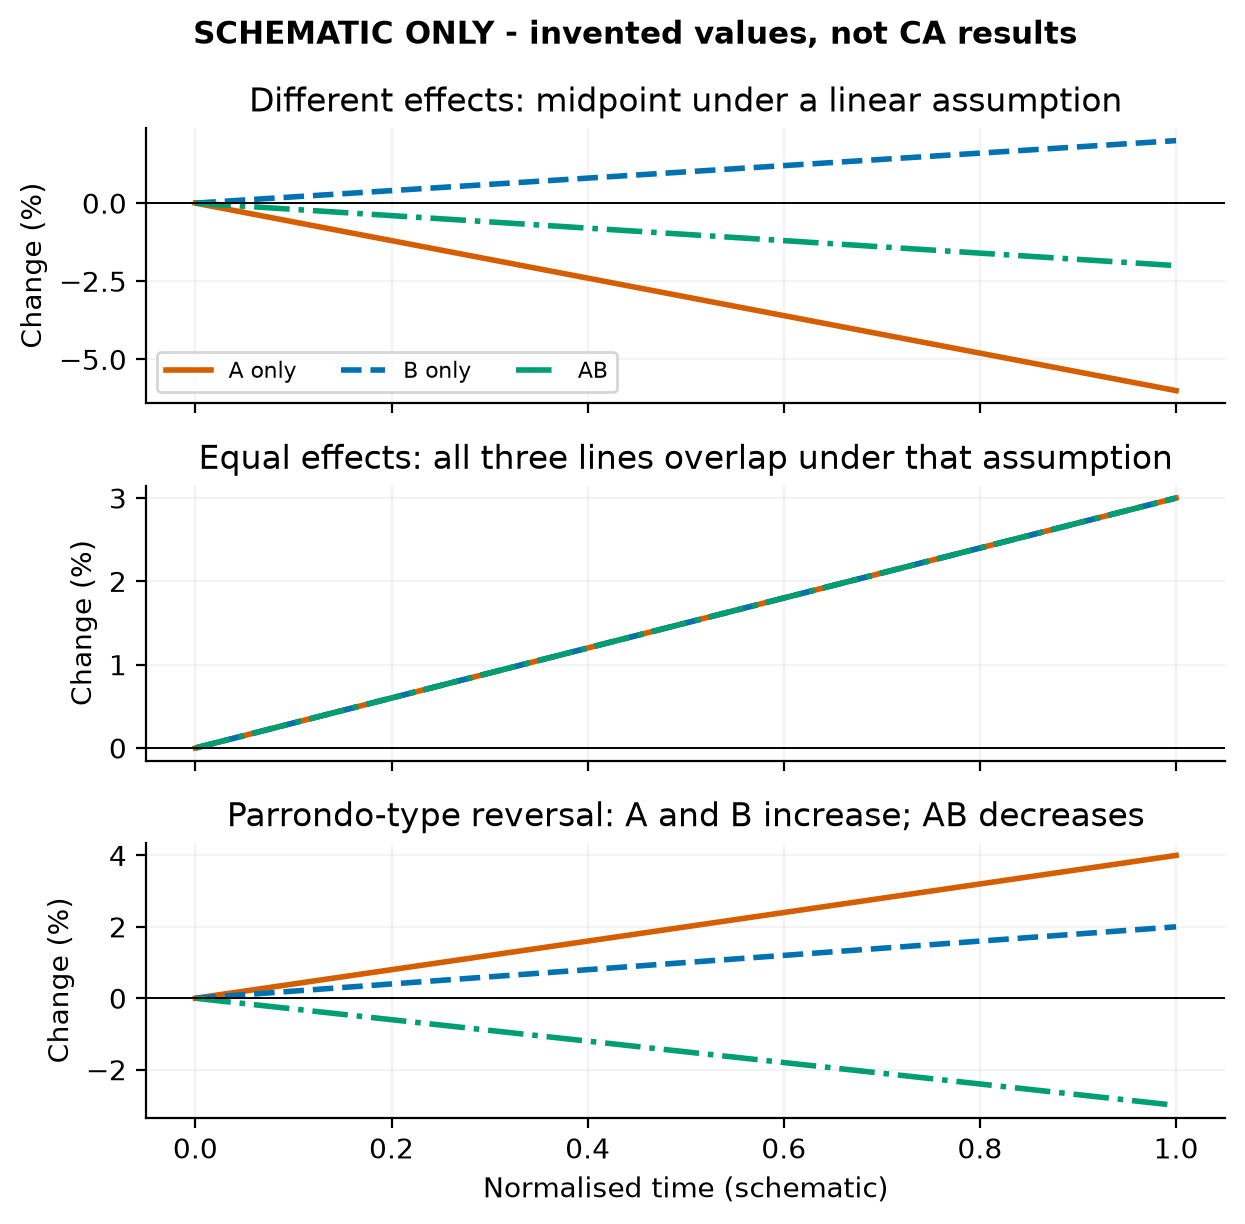
\includegraphics[width=\linewidth,height=0.72\textheight,keepaspectratio]{schematic.png}
\caption{Schematic intuition and a Parrondo-type reversal. All values and straight lines are invented examples, not CA results. The first two panels assume independent, additive treatment effects. The final panel illustrates the required sign reversal. Baseline does not enter that criterion.}\label{fig:schematic}
\end{figure}\clearpage

\begin{figure}[!ht]
\centering
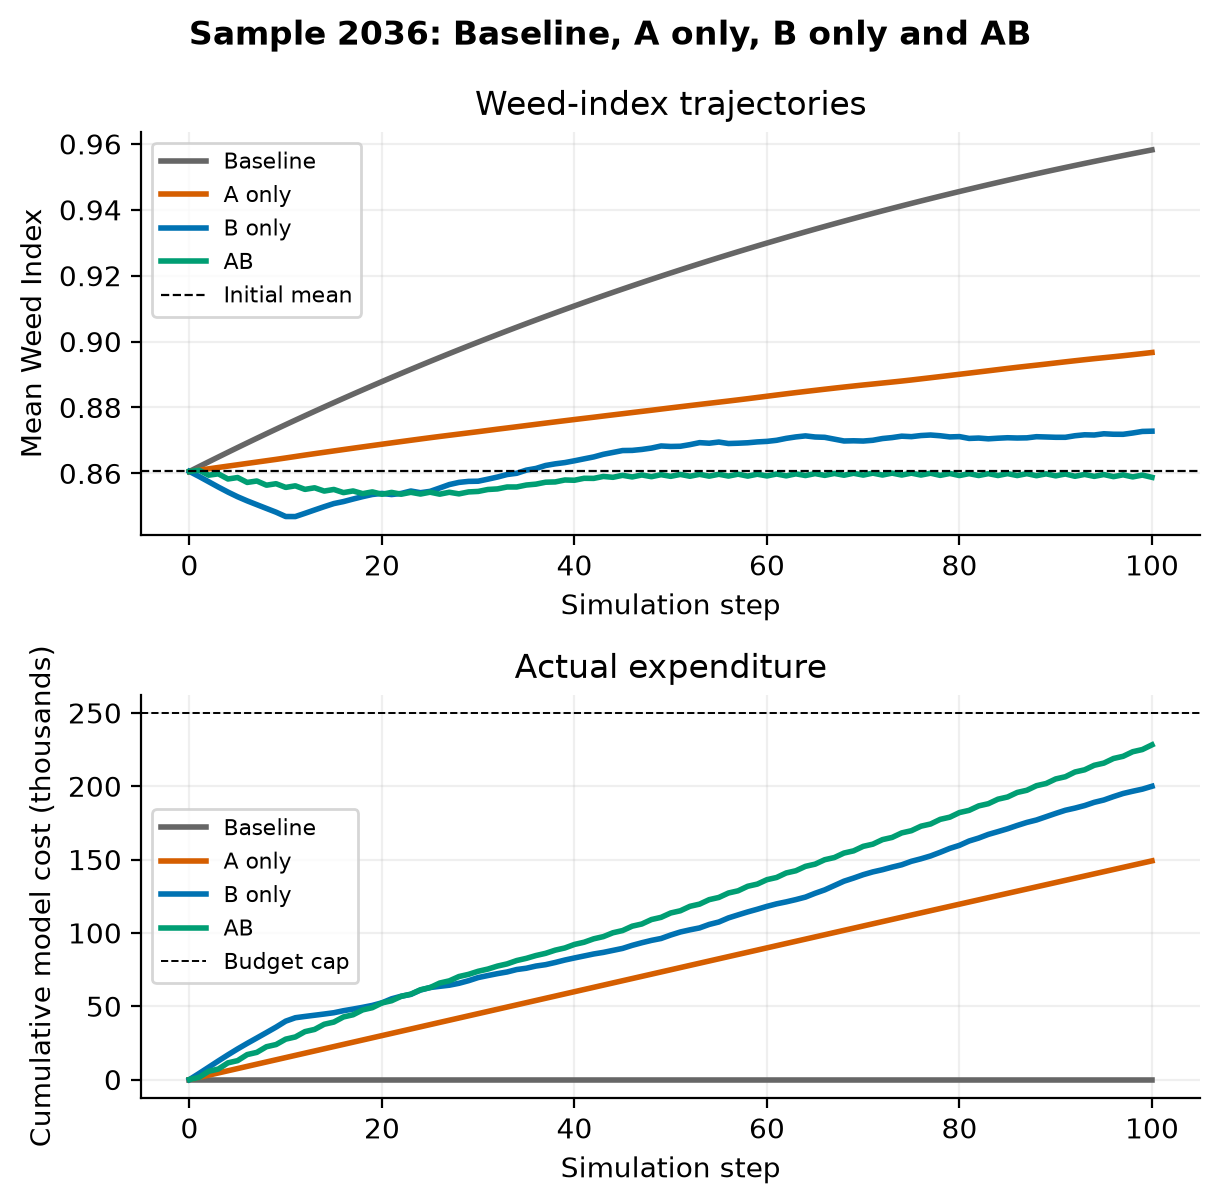
\includegraphics[width=\linewidth,height=0.72\textheight,keepaspectratio]{four_strategies.png}
\caption{Sample 2036 (Step 08): Baseline, A only, B only and AB. Actual results use 1 km cells, 100 steps and a common treatment cap of 250,000 model-cost units. No treated strategy exhausts the cap. The dashed initial-mean line marks the sign-test boundary. AB ends slightly below it, while A and B end above it. Parameters are given in Section 4.1.}\label{fig:actual}
\end{figure}\clearpage

\section*{Appendix B. Tables and Reproducibility}

\subsection*{Table B1. Values represented in the stored parameter search}

\begin{center}\renewcommand{\arraystretch}{1.15}\begin{tabular}{@{}p{.32\linewidth}p{.63\linewidth}@{}}\toprule

Parameter & Values \\

\midrule

A removal fraction & 0.05-0.50 in increments of 0.05 \\

B removal fraction & 0.10-0.80 in increments of 0.05 \\

Maximum cells per call & 25, 50, 75, 100, 150, 200, 300 \\

Density boundary & 0.55-0.90 in increments of 0.05 \\

B lower threshold & 0.05-0.50 in increments of 0.05 \\

Growth rate & 0.010, 0.015, 0.020, 0.025, 0.030, 0.035, 0.040 \\

Propagation rate & 0.0025, 0.005, 0.010, 0.015, 0.020, 0.030 \\

Budget cap & 150,000-450,000 in increments of 50,000 \\

\bottomrule\end{tabular}\end{center}

The CSV contains 2,400 evaluated combinations, not the Cartesian product of this table. Fixed settings are 100 steps, 1 km cells, $K=1$, initial bounds 0.05 and 1, population coefficient 0.000783 and unit removal cost 200.

\subsection*{Table B2. Main four-strategy comparison at 100 steps}

\begin{center}\renewcommand{\arraystretch}{1.15}\begin{tabular}{@{}lrrrr@{}}\toprule

Strategy & Final mean & Change & Actual cost & End step \\

\midrule

Baseline & 0.958180 & +11.342\% & 0 & Not applicable \\

A only & 0.896682 & +4.196\% & 149,107 & Not reached \\

B only & 0.872800 & +1.421\% & 199,967 & Not reached \\

AB & 0.858799 & -0.206\% & 228,213 & Not reached \\

\bottomrule\end{tabular}\end{center}

Initial mean: 0.860575. Costs are model units, not calibrated currency. The untreated Baseline does not consume a budget.

\clearpage

\subsection*{Table B3. Targeted checks on the selected candidate}

\begin{center}\renewcommand{\arraystretch}{1.15}\begin{tabular}{@{}lrrr@{}}\toprule

Setting & A only & B only & AB \\

\midrule

Original, 100 steps & +4.196\% & +1.421\% & -0.206\% \\

No propagation, 100 steps & -1.421\% & -0.068\% & -2.998\% \\

Matched lower expenditure & +6.046\% & +6.340\% & +6.460\% \\

156 steps, proportional cap & +6.362\% & +2.285\% & +0.389\% \\

\bottomrule\end{tabular}\end{center}

Entries are final changes from the common initial mean. Matched expenditure is approximately 124,279 units for all three treated strategies, using Step 14's cap based on the smallest expenditure across six original schedules. The 156-step comparison uses a cap of 390,000, preserving the original cap per step. All rows concern sample 2036.

The source search is \url{results/strong_parrondo_equal_budget_search.csv}. Sample 2036 is the candidate in \url{notebooks/experiments/step08_parrondo_strong_condition_validation.ipynb}. The consolidated \url{notebooks/demonstration.ipynb} contains the simulation, figure-export and additional comparison cells. Running its main comparison and figure cells regenerates Figures A1--A2 in \url{report/sample2036/}; Figure A1 is explicitly schematic. The main results are stored in that directory's summary, trajectory and cost CSV files. Saved follow-up evidence is in the Step 10--14 result CSV files under \url{results/}, filtered to sample 2036. The project repository is \url{https://github.com/RayYouDS/cits4403-parrondo-weed-control}.

\clearpage
\section*{Appendix C. AI Use Statement}

The authors wrote the core code themselves and used GPT-5.6 (OpenAI) to assist with debugging and refinement. They sought AI suggestions when considering improvements, while making the final decisions about the model, experiments and interpretation themselves. AI assistance also supported analysis scripts, plots and LaTeX formatting during report preparation.

For the report, the authors established the overall direction and prepared the initial content. They then refined the structure, wording and clarity through dialogue with AI, including assistance with English expression and translation. The authors reviewed the resulting content and proceeded on the basis of their own understanding and judgement. AI was used as a supporting tool, and the authors remain responsible for the submitted code, results, references and conclusions.

\end{document}
